
%%%%%%%%%%%%%%%%%%%%%%%%%%%%%%%%%%%%
%						Deep Neural Network 
%
%	 Author: Valgi0
%
%  Goal: All notes from various sources 
% 
%%%%%%%%%%%%%

\documentclass[12pt,a4paper,twoside,openright]{scrbook}

\usepackage[utf8]{inputenc}
\usepackage[english]{babel}
\usepackage[T1]{fontenc}


\usepackage{amsmath,amsfonts,amssymb,amsthm}
\usepackage{caption}
\usepackage[usenames]{color}
\usepackage{enumerate}
\usepackage{fancyhdr}
\usepackage{fancyvrb}
\usepackage{float}
\usepackage{graphicx}
\usepackage{booktabs}
\usepackage{indentfirst}
\usepackage{listings}
\usepackage{marvosym}
\usepackage{multicol}
\usepackage{sectsty}
\usepackage{subcaption}
\usepackage{tocloft}
\usepackage{microtype}
\usepackage[table]{xcolor}
\usepackage{url}
\usepackage{hyperref}
\usepackage{adjustbox}
\usepackage{blindtext}


\hypersetup{%
	pdfpagemode={UseOutlines},
	bookmarksopen,
	pdfstartview={FitH},
	colorlinks,
	linkcolor={black},
	citecolor={black},
	urlcolor={black}
}


\makeindex

\subject{my note about}
\title{Basic (and Maybe advanced) Deep Learning stuff }
\subtitle{theory and samples}
\author{Valgi0 (me as always)}

\begin{document}

\frontmatter 

\maketitle


\newpage

\tableofcontents

\newpage

\listoffigures

\mainmatter

\pagestyle{fancy} 
\fancyhead[LO]{\nouppercase{\rightmark}}
\fancyhead[RE]{\nouppercase{\leftmark}}
\fancyhead[LE,RO]{\thepage}
\fancyfoot{}

%% CAPITOLO 1
\chapter{Why this documents}
I feel the exigence to put together all my notes and my experience in this wide word of Deep Neural Network. I want them in one place with a good organization allowing me and the reader to access to what I need quickly. This thought came to my mind while I was working to my dissertation thesis, and for the haste, I used to write notes every where and when I needed them they were hard to find. Btw I don't care to write why I'm doing this so

\section{Where Information come from}
I'm going to use some books freely distributed and one day I'll put the links here. Stay tuned

\section{Chapters organization}
Each chapter contains arguments to one topic and information are organized following this schema:
\begin{itemize}
\item Introduction to the topic
\item Theory about topic
\item Examples maybe
\item Related links or papers ( Idk )
\end{itemize}

\section{Notation}
\begin{itemize}
\item \textit{a,b,c} are scalars
\item \textbf{a,b,c} are vectors
\item \textbf{A,B,C} are matrices
\item \textbf{0} it is a zero vector
\item $P(x=x_i), x \sim P(x_i)$ Probability mass function over a discrete variable $x$
\item $p(x=x_i), x \sim p(x_i)$ Probability density function over a discrete variable $x$ where $x_i$ is a range of value
\item $x \perp y$ the two variables are independent
\end{itemize}

\chapter{Has someone said Math?}

In this chapter we are going to explore all math stuff we need to fully understand the concepts.
If God Exists he must be a mathematician.

\section{Linear Algebra OMG}

Let's start by defining what is a vector.. a vector is a vector. $\textbf{v} = [i_0, i_1, i_2, ... , i_n]$. In this case $v$ is a vector composed by elements $i \in \mathbb{I}$ with size $n$. So vector comes from $\mathbb{R}^n$ space. This is the n-dimensional Euclidean Space. A vector with all zeros is called \textbf{zero vector} and it will be represented as $\textbf{0}$

\subsection{Vector Space}
The Vector Space $\mathbb{X}$ is a set of vectors that satisfies the following conditions:
\begin{itemize}
\item \textbf{Addition Closure}. This means that:
\begin{itemize}
 \item if $\textbf{x}, \textbf{y} \in \mathbb{X}$ so $\textbf{x} + \textbf{y} = \textbf{j}$ and $\textbf{j} \in \mathbb{X}$ for each $\textbf{x,y}$
 \item  $\textbf{x} + \textbf{y} = \textbf{y} + \textbf{x}$
 \item  $\textbf{x} + (\textbf{y} + \textbf{c}) = (\textbf{x} + \textbf{y}) + \textbf{c}$
 \item $\textbf{x} + \textbf{0} = \textbf{x}$
 \item For each $x \in \mathbb{X}$ exists a unique vector called $\textbf{-x}$ such that $\textbf{x} + (\textbf{-x}) = \textbf{0}$
 \end{itemize} 
\item \textbf{Multiplication Closure}. This means that if $\textbf{x} \in \mathbb{X}$ and $y$ a scalar so $\textbf{x} * y = \textbf{j}$ and $\textbf{j} \in \mathbb{X}$ for each $\textbf{x,y}$ \begin{itemize}
\item $\textbf{x} * 1 = \textbf{x}$
\item For any $a, b$ scalars $(ab)*\textbf{x} = a(b*\textbf{x})$
\item $(a + b)*\textbf{x} = a*\textbf{x} + b*\textbf{x}$
\item $a(\textbf{x} + \textbf{y}) = a*\textbf{x} + a*\textbf{y}$
\end{itemize}
\end{itemize}

From the above conditions we can extract some considerations. The first is that each $\mathbb{R}^n$ is a vector space. A subset of this euclidean space can be a vector space only if it his unbounded. For example:
\newline
\[ \mathbb{X} = ( (x,y) : x < 5  y < 5, (x,y) \in \mathbb{R}^2)\] \newline \[
v_0 = (4,4), v_1 = (3,3) \in \mathbb{X}\] \newline \[
v_0 + v_1 = v_2 = (7,7) not \in \mathbb{X}
\]
So $\mathbb{X}$ is not a vector space.

\subsection{Linear Independence}
\textbf{Linear combination} is a very cool stuff. Let's have a vector $\textbf{x}$ and some different vectors $\textbf{y,z,k}$. If there exists a set of three scalars such that $a_0*\textbf{y} + a_1*\textbf{z} + a_2*\textbf{k} = \textbf{x}$ so $a_0*\textbf{y} + a_1*\textbf{z} + a_2*\textbf{k}$ is a linear combination.
Linear indipendence is a propery between more vectors. $\textbf{x}_0, \textbf{x}_1,...,  \textbf{x}_n$ are linearly dependent  just if there exist $n$ scalars at least one of which is not zero, that:
\[a_0\textbf{x}_0 + a_1\textbf{x}_1 +  ... + a_n\textbf{x}_n = \textbf{0} \]
Otherwise, if all $a_i$ are 0, vectors are \textit{linearly independent}.
\textbf{Attention} if a set of vectors is linearly dependent so one or more that tis vectors can be obtained by a linear combination of others.
\newline
\textbf{Let's do some examples}
\[\textbf{v}_0 = [1,-1], \textbf{v}_1=[-1,1] , \textbf{v}_2 = [-1,-1]\]
These are three vectors. Are they linearly independent?
\[a_0*\textbf{v}_0  +  a_1*\textbf{v}_1 + \textbf{v}_2*a_2  = 0 \rightarrow \begin{bmatrix}
 a_0 - a_1 - a_2 = 0 \\ -a_0 + a_1 - a_2 = 0
\end{bmatrix} \]
Now we need to solve those equations:
\[a_0 = a_1, a_2 = 0\]
So they are a linear dependent vectors. This means that we can select one of them and express it as a linear combination of the others:
\[\textbf{v}_0 = \textbf{v}_1*a_1 + \textbf{v}_2*a_2\]
That is true for $a_1 = -1$ and $a_2 = 0$.

\subsection{Spanning a Vectors space}
To create a vector space we can grab some vectors and create this space as the set of all linear combinations of these vectors. It the given vectors are linearly independent they are called \textbf{Basis set} for that vector space. The number of vectors in the basis set is the dimension of the vector space. This means that we can express each vector inside that space using a number of independent vectors equal to the dimension of the space.\newline
\textbf{For Example} $\mathbb{R}^2$ can have as basis $(1,0), (0,1)$. Using these two vectors we can create each vector inside the space. Try to believe.

A vector space can have infinite basis. But the basis composed by binary vectors

\subsection{Some functions}
Some functions can be defined between vectors. the first is the \textbf{Inner Product} that is the product between two vector and it is represented with $(\textbf{x}, \textbf{y})$. This function must follow these properties:
\begin{itemize}
\item $(\textbf{x}, \textbf{y}) = (\textbf{y}, \textbf{x})$ 
\item $\textbf{x} (a \textbf{y} + b \textbf{j}) = a(\textbf{x}, \textbf{y}) + b(\textbf{x}, \textbf{j})$
\item $(\textbf{x}, \textbf{y}) \geq 0$ if $\textbf{x}$ is not the zero vector.
\end{itemize}
The standard inner product adopted the respect the above properties is:
\begin{equation}
\textbf{x}\textbf{y} = x_{0}y_{0} + x_{1}y_{1} + ... + x_{n}y_{n}
\end{equation}

Another function that can be defined is the \textbf{Norm} represented by $\parallel \textbf{x} \parallel$. This function must respect these properties:
\begin{itemize}
\item $\parallel \textbf{x} \parallel \geq 0$
\item $\parallel \textbf{x} \parallel = 0$ if $\textbf{x}$ is the zero vector
\item $\parallel a\textbf{x} \parallel = \mid a \mid \parallel \textbf{x} \parallel$
\item $\parallel \textbf{x} + \textbf{y} \parallel \leq \parallel \textbf{x} \parallel + \parallel \textbf{y} \parallel$
\end{itemize}
There are many function that satisfy these conditions. The most common \textbf{norm} is:
\begin{equation}
\parallel \textbf{x} \parallel = (\textbf{x}\textbf{x})^{\frac{1}{2}} = \sqrt{x_0^2 + x_1^2 + ... + x_n^2}
\end{equation}

Using both of the previous function we can define the \textit{angle} between two vectors. In particular we can calculate the \textit{cosine}:
\begin{equation}
cosine(\textbf{x},\textbf{y}) = \frac{ \textbf{x}\textbf{y}}{\parallel \textbf{x} \parallel \parallel \textbf{y} \parallel}
\end{equation}
 
 \section{Linear Transformation}
 For \textbf{Transformation} we identify the operation that relate a value x to a value y. Let's define:
 \begin{itemize}
 \item \textit{Domain} the set of $x_i \in \mathbb{X}$ values.
 \item \textit{Range} or Co-domain the set of $y_i \in \mathbb{Y}$ values
 \item \textit{Transformation} as the rule relating each $x_i$ to an $y_i$ 
 \end{itemize}
 
 A transformation $A$ is \textit{Linear} if:
 \begin{itemize}
 \item for all $x_0, x_1$ $A(x_0 + x_1) = A(x_0) + A(x_1)$
 \item for all $x_0$ and for all $a$ scalars $A(x_0*a) = A(x_0) * a$   
 \end{itemize}
 
 \textbf{IMPORTANT}\\
 \emph{For any transformation between two finite dimensions vector space can be represented by a Matrix. This Matrix is build using the basis of the vector spaces so changing them the matrix change}
 
 \subsection{Eigenvalues eigenvectors}
 All vectors from a Vector space not $0$ and scalars that make this equation true:
 \begin{equation}
 A(\textbf(z)) = a\textbf(z)
\end{equation}  
are called Eigenvalues and eigenvectors. 
What that means?? Graphically the eingenvector of a Linear transformation is the direction for which vectors in that direction that after the transformation will have the same direction but a different length.

\subsubsection{How to compute them}
In order to compute them let's  take a look to the formula:
\[ A(\textbf{z}) = a\textbf{z} \]
We said that a linear transformation can be represented by a matrix so the formula becomes:
 \[ \textbf{A}\textbf{z} = a\textbf{z} \]
 \[(\textbf{A} - a\textbf{I}) * \textbf{z} = 0\]
 Let's define \textbf{A} matrix as:
 \[\begin{vmatrix}
-1 & 1\\0 & -2 
 \end{vmatrix}\]
 so $(\textbf{A} - a\textbf{I}) = 0$ (Now we look for determinant that is 0,.. dont ask why) is:
  \[\begin{vmatrix}
-1 - a & 1\\0 & -2 - a
 \end{vmatrix} = 0 \]
The solutions are found solving:
\[a^2 + 3a + 2 = (a + 1)(a + 2) = 0 \Rightarrow a_0 = -1 a_1=-2\]
Those are the eigenvalues. To find the vectors you must solve the equation \[(\textbf{A} - a\textbf{I}) * \textbf{z} = 0\] using each eigenvalue.

\section{Probability}
Let's talk about probability. In machine learning and Deep learning probability is essential cause the are stochastic fields and not deterministic ones. Let's define a variable $x_r$ as a random variable on a dice domain. This means that it can be each value within 1,2,3,4,5,6 with the same probability. 

Let's speak about \textbf{Probability Mass Function} as the probability that some variables can be found in a certain state.
For example $P(x_r = 1) = 1/6$ (For completeness it's possible to write this function in other ways: $x_r \sim P(1)$ or $P_{x_r}(1) $. 

We can have more dices and we can define  \textbf{Joint Probability} as a Probability Mass Function defined on more variables: $P(x_r = 1, y_r = 2)$ that denotes the probability that $x_r = 1$ and $y_r = 2$ at once.

$P(x)$ must follow some properties:
\begin{itemize}
 \item $\forall x_i \in x_r 0 < P(x_i) < 1$
 \item $\forall x_i \in x_r \sum P(x_i) = 1  $
 \end{itemize} 
 
 But htis works for discrete variable, for continuous variable defined on $\mathbb{R}$ things become harder. We define the probability to find the variable in a range of value. Let's define the range as $[a,b]$ with $a,b \in \mathbb{R}$ and $b>=a$. Let's define $p$ the \textbf{Probability density function} as the function that denotes the probability of the input variable to be found with a value in the given range: $p(x_r; a, b)$. This function draws a linear function that must follow some properties:
 \begin{itemize}
  \item Area beneath the function must be 1: $\int p(x)dx = 1$
  \item $p(x) >= 0$ 
  \end{itemize} 
  
  \subsection{Conditional Probability}
  
  Let's define two events $x_0, y_0$ and for some reason they are connected in some way. Now we want to compute the probability of $y_r = y_0$ knowing that  $x_r = x_0$ has happened. In this case we speak about \textbf{Conditional Probability} and it's defined: 
  \begin{equation}
    P( y_r = y_0|x_r = x_0) = \frac{P( y_r = y_0, x_r = x_0)}{P(x_r = x_0)}
  \end{equation}
  
  
 For examples let's use ours dices. We want to know the probability to get $y_r = 1$ if we already got $x_r = 1$. 
 So $P(1 | 1) = \frac{P(1, 1)}{P(1)}$ in this case we get: $\frac{1/36}{1/6} = \frac{6}{36} = \frac{1}{6}$ what we get in this case is the two dices are independent, the probability to have 1 in the second dice doesn't change respect the first.  
 
 Some times we know the probability of $P(x|y)$ and the probability of $P(x)$. We would like to know the probability of $P(x|y)$. To get that we can use the \textbf{Bayes' Rule}: 

\begin{equation}
 P(x_r = x_0 | y_r = y_0) = \frac{P(x_0)P(y_0 | x_0)}{P(y_0)}
\end{equation} 

 It's time to do some exercises.
 \paragraph{Exercise}
 Let's have Robert a funny boys who is going to get a dog. In the shop there are 6 dogs: 4 males and 2 females and the shopper has to chose the dog for him randomly. Furthermore he has already thought about names: if dog is male the name is one of: Spike, Mike, Andy. Otherwise, if the animal is female, the name could be: Sally or Andy.
 In this situation we want to know the probability the dog will be called Sally, the probability that if the dog was called Andy it would be male.

First we need compute the probability to get a dog named Sally:

\[P(name = Sally) = P(dog = male)*P(name=Sally | dog=male)  = 4/6 * 1/2 = 1/3\]

$P(dog = male | name = Andy)$ for this case we have to use Bayes' Rule:

$\frac{P(dog=male)P(name = Andy | dog = male)}{P(name = Andy)}$.

We need the probability $P(name=Andy)$ and it is:

 $P(dog=male)*P(name=Andy | dog=male) + P(dog=female)*P(name=Andy | dog=female)  = 7/18$

 Let's resolve this:

$\frac{4/6 * 1/3}{7/18} = 2/9 * 18/7 = 4/7$

\subsection{Chain rule of probability}

The chain rule let us decompose a joint distribution in a conditional distributions over only one variables.
For examples we have 3 discrete variables:

$P(a,b,c) $ can be rewritten over $c$: $P(c) * P(b|c) * P(a | b,c)$

We can generalize this property using this formula:

\begin{equation}
P(x_0, ..., x_n) = P(x_0) \prod_{i = 1}^n P(x_i | x_0, ... , x_{i-1})
\end{equation}

That is. Nothing more and nothing less

\subsection{Marginal Probability}

Let's imagine we have a set of discrete variables $x_0, ... , x_n \in \mathbb{S}$ and we know the probability distribution over them. Now we want to know the probability distribution over a subset of them $x_k, .. , x_m \in \mathbb{S}'$. This distribution is called \textbf{Marginal distribution} and can be calculated using the \textbf{sum rule}:
\begin{equation}
\forall x_i \in \mathbb{S}', P(x_i) = \sum_{x \neq x_i \in \mathbb{S}} P(x_0, ... , x_i, ..., x_n)
\end{equation}

For continuous variables the formula exploits the derivatives. Let's imagine we have two variable $x,y$:
\begin{equation}
p(x) = \int p(x, y)*dy
\end{equation}

\subsection{Relationships between variables}
Let's have two variables $x,y$. We can say they are \textbf{independent} if  their probability distribution can be expressed as the product of the tow factors:
\begin{equation}
 p(x = x_i, y = y_i) = p(x = x_i)p(y=y_i) \forall x_i, y_i 
 \end{equation} 
 
 we also can say they are \textbf{Conditional Independent} if  given a event $z$ the probability distribution can be factorized as:
 
 \begin{equation}
 p(x = x_i, y = y_i | z ) = p(x=x_i | z) p(y=y_i | z)
 \end{equation}
 
 If two variable are are independent we can denote that using: $x \perp y$. \linebreak
 If two variable are conditional independent we can denote that using   $x \perp y | z$



\chapter{Let's start}

In this chapter we are going to see the very basic of Neural Network like \textit{Neurons}, \textit{Links}, \ldots.

\section{Single Neuron}
Neuron is the basic unit of Neural Network and is just a mathematical function applied to an input.
Let's define an input a scalar \textit{i} a scalar weight \textit{w}, a scalar bias \textit{b} and a function \textit{f}.
Neuron function is:
\begin{equation}
a = f(iw + b)
\end{equation}
Function \textit{f} is called \textbf{Activation Function} or sometimes \textbf{Transfer function} and usually is a non linear function.

\subsection{Example of neuron}
\textit{i} = 5, \textit{w} = 0.5, \textit{b} = 2 and \textit{f(x)} = $x + 1$  
\begin{equation}
f(5*0.5 + 2) = f(4,5) = 5.5
\end{equation}

\section{Transfer functions}
\begin{figure}
    \centering
    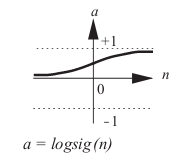
\includegraphics[scale=0.65]{img/log-sigmoid-function.png}
    \caption{log-sigmoid function}
    \label{img:log-sigmoid}
\end{figure}{}
Or Activation function are chosen during model creation in fact they are Hyper-Parameters. They can be linear or non-linear. Now some of the most important linear functions are listed:
\begin{itemize}
\item \textbf{Hard Limit Transfer Function}. This function produce 0 if input value is negative or 1 if value is equal or greater that 0. It creates a step and it is used for binary classification problems
\item \textbf{Linear Function}. $f(x) = x*m +q$. It is the function of the line.
\item \textbf{log-sigmoid transfer function}. $f(x) = \frac{1}{1+e^{-x}}$. This function produce a value always positive and you can see the graphic at the figure \ref{img:log-sigmoid}
\end{itemize}
\begin{figure}
    \centering
    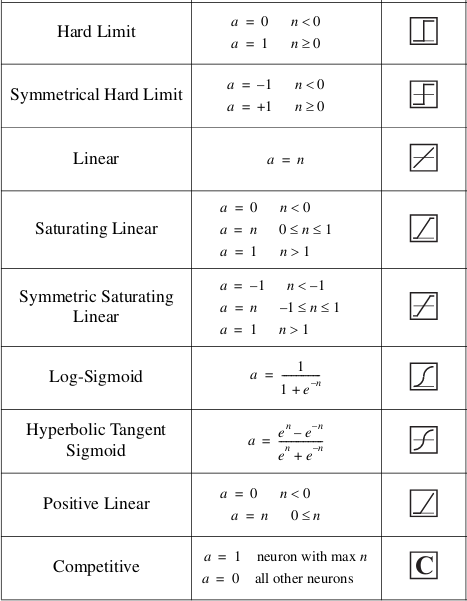
\includegraphics[scale=0.65]{img/activation-functions-table.png}
    \caption{Overview of basic activation functions}
    \label{img:activation-functions-basic}
\end{figure}

\subsubsection{Diagonalization}

A matrix that represents a linear transformation can be \textit{Diagonilized} by changing the basis in the one composed with only Eigenvectors. Each dimension is represented by one of those vectors so the matrix has to contain all eigenvalues to perform such operation. In this way it become a diagonal matrix filled by eigenvalues. 

\section{Multi-input Neuron}
Usually neuron has more than one input at time. Each of them want a private \textit{w} while \textit{b} the bias is one for all. Under this light we can say that input \textbf{i} is a column vector of $i_0,.., i_n$ elements and neuron contains a scalar \textit{b} and a vectors of \textbf{w} of n weights. Using \textit{f} as linear function $f(x) =x + 1$ the neuron perform this equation:
\begin{equation}
a = f(\textbf{wi} + b) = f((\sum_{j=0}^{n} w_j * i_j) + b)
\end{equation}

\subsection{Example}
\textbf{i} = $5,6,7$ \textbf{w} = $1,2,-1$ \textit{b} = 2 and \textit{f(x)} = $x + 1$  
\begin{equation}
f(5*1 + 6*2 + 7*-1 + 2) = f(12) = 13
\end{equation}

\section{Multi-neurons}
Often Input vector goes to multiple neurons and these neurons are a Layer. It is important keep in mind that:
\begin{itemize}
\item All Neurons take all input. So \textit{w} weights is a vector with the same dimension of the input vector
\item All Neuron produce a scalar so the number of neurons in a layer is the number of  outputs.
\item Each neuron has its bias so a layer has a vector of bias one per neurons 
\end{itemize}

Let's define input \textbf{i} a column vector and weight \textbf{W} as a matrix $m*n$ where $m$ is the number of the neuron and $n$ the number of the input elements in \textbf{i}. \textit{f} is the activation function:

\begin{equation}
\textbf{a} = f(\textbf{W}\textbf{i} + b)
\end{equation}

From the above equation we can see that a matmul is performed between weights matrix and input column vector. So row $j$, that is the weight vector of the neuron $j$ is multiplied and summed with the whole input column vector.

\begin{equation}
  \begin{bmatrix}
w_{0,0} & w_{0,1} & \ldots & w_{0,n} \\
w_{1,0} & w_{1,0} & \ldots & w_{1,n} \\
\vdots & \vdots & \vdots & \vdots \\
w_{m,0} & w_{m,1} & \ldots & w_{m,n} \\
  \end{bmatrix} * \begin{bmatrix}
  i_0 \\ i_1 \\ \vdots \\ i_n
  \end{bmatrix}
\end{equation}

So a neural layer can be seen as a matrix of weight and a Bias vector:
\begin{equation}
Layer_w = \begin{bmatrix}
n_0 \\ n_1\\ n_2\\ \vdots \\ n_m
\end{bmatrix} = \begin{bmatrix}
w_{0,0} & w_{0,1} & \ldots & w_{0,n} \\
w_{1,0} & w_{1,0} & \ldots & w_{1,n} \\
\vdots & \vdots & \vdots & \vdots \\
w_{m,0} & w_{m,1} & \ldots & w_{m,n} \\
\end{bmatrix}
\end{equation}
\begin{equation}
Layer_b = [b_0, b_1, b_2, \ldots , b_m]
\end{equation}

Mathematically a layer can be represents just by \textbf{W} the weight matrix and \textbf{b} the bias vector.

\section{Multi Layers}

A neural network has more layers. The first layer is called \textbf{Input layer} the last in called \textbf{Output layer} and the ones in the middle are \textbf{Hidden Layers}. 
Each layers can have different number of neurons and different activation function. So a basic multi-layer network with $l$ layers is defined by $f_0, ..., f_l$ activation functions, $\textbf{W}_0,..., \textbf{W}_l$ weight matrices and $\textbf{b}_0,...,\textbf{b}_l$ or just \textbf{B} bias (matrix contains in row $j$ the bias vector for the layer $j$).
This network take inputs with the first layer, generate output and then gives this output to the second layer and so on.
A Multi layer Network performs:
\begin{equation}
\textbf{a} = f_l(f_{l-1}(\ldots * \textbf{W}_{l-1} + \textbf{b}_{l-1}) * \textbf{W}_{l} + \textbf{b}_{l})
\end{equation}

This Multi-layer neural Network is called \textbf{Feed Forward Neural Network}

\section{Recurrent Neural Network}
Feed forward neural network has layers and layer has neurons. Each Neuron take a input vector \textbf{i} and produce a scalar \textit{a}. Differently, Recurrent Neural Network takes two input vector the input vector \textbf{i} and some \textit{a'} that is the output of the previous input. Let's imagine we have a time series of data $i_0,...,i_t$. This data must be given to the model respecting the sequence but we want model somehow remember previous data. For this kind of task Recurrent Neural Network was created. They have layers and neurons but each neuron has two vectors and a bias: \textit{u} weights for the input, \textit{w} weights for its layer output at the previous step and \textit{b} the bias. Let me explain in a intuitive way before using math: the input is a series of vectors. First vector $i_0$ is taken and is given to the first layer of the model. Each neurons of this layer get the input vector $i_0$ and produce a scalar $a_0$ and with other neurons output of that layer it creates the layer output \textit{a}  Nothing new until now. Output goes to the second layer and so on until last layer. Second input is taken $i_1$ and neuron  receives it and the previous layer output \textit{a}. Using both of them it compute the next scalar output $nexta_0$. And so on! 

Let's define its behavior using some cool math. Our network is composed by 1 layer with 1 neuron:
\begin{equation}
  inputsequence= \textbf{i}_0, \ldots ,\textbf{i}_k 
\end{equation}
\begin{equation}
  f_{neuron} = ActivationFunc( b + \textbf{w}*a'_{t - 1} + \textbf{u}*\textbf{i}_t) = a_{t}
\end{equation}
The neuron takes at time t in input $a'_{0,t - 1}$ and $i_{0,t}$ and produce $a_{t}$. In this case with just one neuron the layer output coincide with the neuron output. After that the following equation is performed to compute $a'_t$
\begin{equation}
a'_t = c + \textbf{v}a_t
\end{equation}

Let's imagine to have a Recurrent Neural Network with more layers and more neurons for each layers. The above equations become:
\begin{equation}
\textbf{a}_t = ActivationFunc(\textbf{b} + \textbf{W}*\textbf{a'}_{l,t-1} + \textbf{U}*\textbf{i}_t)
\end{equation}
$a'_{l,t-1}$ means the column vector output from the layer $l$ at time step $t-1$
\begin{equation}
\textbf{a'}_{l,t} = \textbf{c} + \textbf{V}\textbf{a}_{l,t} 
\end{equation} 

That is all my dear.. Not true, we are going to expand this kind of network later

\subsection{Keep in mind}
Some tips to keep in mind when you work with Recurrent Neural Network
\begin{itemize}
\item Externally are similar to feed forward network.. it has layers and neurons
\item The inputs are sequence of inputs vectors
\item Output is a series of vectors one for each inputs vector but if a prediction is what u want last output must be used.
\item At any time neuron takes exactly 2 input vectors in input and they are the output from prior layer and output for its layer but a time t-1. 
\item For each input vectors neurons has a weight vector this means that a layer has a \textbf{W} and \textbf{U} weight. The first for its own output and the second for the output of the previous layer.
\item Output of a layer is turned in a input performing $c + \textbf{V}a_l$ where c is a bias and \textbf{V} is a weight matrix.
\end{itemize}

\section{Some Applications}
In this section we are going to see how the previously explained network are used in a very easy problem:
\emph{
We have some fruits composed by oranges and apples and we need a model capable to tell us if a given fruit is one or it is the other. Fruits is defined by size, dimension, weight.
}

Let be $i_a = \begin{vmatrix}
1 & -1 & -1
\end{vmatrix}$ the vector that represent an apple and  $i_o = \begin{vmatrix}
1 & 1 & -1
\end{vmatrix}$ the one that represent an orange. 

\subsection{Perceptron}
Perceptron is a binary classifier based on single layer \textbf{Feed Forward Network} with \textbf{Hard Limit} as activation function. So if the output is minor than 0 the function produces 0 otherwise 1.

\begin{equation}
output = HardLims(\textbf{W}\textbf{i} + \textbf{b})
\end{equation}

\textbf{W} is a matrix $nxm$ where n is the dimension of the input vector (3 in this case) and $m$ the number of neurons in the layer.

Let's define $W = [0, 1, 0]$ for a single neuron layer. This is called \textbf{Single-Neuron Perceptron}. Now we can test it against our data.
\newline
\textbf{Apple} defined as  $i_a = \begin{vmatrix}
1 & -1 & -1
\end{vmatrix}$ is multiplied by \textbf{W}
\begin{equation}
[0, 1, 0] * \begin{vmatrix}
1 & -1 & -1
\end{vmatrix}^T = 0*1 + 1*-1 * 0*1 = -1
\end{equation}
\textit{For simplicity input vector is not in column but it should be. Don't judge me}
\begin{equation}
hardlims(-1) = -1
\end{equation}
Ok! model classify apple as -1 let's check if orange are classified as 1
\begin{equation}
[0, 1, 0] * \begin{vmatrix}
1 & 1 & -1
\end{vmatrix}^T = 0*1 + 1*1 * 0*1 = 1
\end{equation}
\begin{equation}
hardlims(1) = 1
\end{equation}

OMG!!!! That is amazing... or not but anyway with a weight vector $[0, 1, 0]$ model is able to classify the fruits. Now try with banana and tell me if it works! COME ON!

\chapter{Basic Concepts about learning rules}
In this chapter we are going to study in deep the basic concepts about learning rule. With  \textit{learning rule} it means all the rules and algorithms used to modify the weight and the bias of the network in order to improve the results.
There are three main approaches:
\begin{itemize}
\item \textit{Supervised learning}. In this case the net is trained by using a set of examples composed by $(p_0, t_0)$ where $p_0$ is the input for the network and $t_0$ the corresponding correct result (target). The result produced is compared to the target. The learning rules are used to modify weights to make model produce the right result. 
\item \textit{Reinforcement Learning}. The algorithm produce a score or a grade according to the network performance and the learning rule seek to adjust weights in order to get higher scores. The network continues to learn also during its application.  
\item \textit{Unsupervised Learning}. The data does not have the target but they are somehow clustered. The cluster becomes the target to predict like the one in the supervised learning.
\end{itemize}

Probably, we will speak about all this approaches later.

\section{Learning rules for Perceptron Architecture}

\subsection{Perceptron Network again}
\begin{figure}
    \centering
    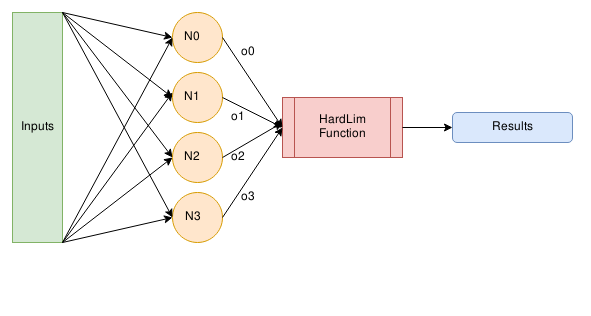
\includegraphics[scale=0.65]{img/PerceptronNetwork.png}
    \caption{Overview of a Perceptron Network}
    \label{img:perceptron_network}
\end{figure}
The perceptron network has a single layer of $S$ neurons and it use as activation function the \textbf{Hardlim} (it produce 0 or 1 according to the output of the neuron).
The weights of the network are:
\begin{equation}
\textbf{W} = \begin{bmatrix}
\textbf{w}_0 \\ \textbf{w}_1 \\ \vdots \\ \textbf{w}_s 
\end{bmatrix}
\end{equation}

So each neuron has a list of $w_{n0}, ... , w_{nm}$ weights where $n$ it the neuron and $m$ is the number of weight and it is the same for the number of inputs.

Each neuron produce a result $o_n$ and the list with all results from all neurons is given to the activation function.

\section*{the decision boundary}
Let's use a Perceptron Network with one neuron and 2 inputs. The result is obtained by this formula:
\begin{equation}
o = hardlim((w_0 * p_0 + w_1 * p_1) + b)
\end{equation}
The decision boundary of the network is determined by the sub set of inputs that make the neurons produce zeros.
\newline
\textbf{Example:}
Let's have $w_0 = 1$, $w_1= 1$ and $b = -1$. So the decision boundary will be:
\begin{equation}
(w_0 * p_0 + w_1 * p_1) + b = p_0 + p_1 - 1 = 0 \Rightarrow p_0 + p_1 = 1
\end{equation} 

The decision boundary define a line in the input space. On one side of that line, the network output will be 0, on the other side will be one.
\begin{figure}
    \centering
    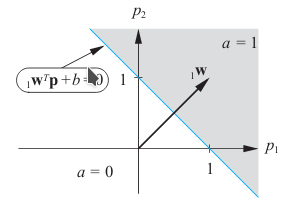
\includegraphics[scale=0.5]{img/decision_boundary_for_perceptron.png}
    \caption{Graphic representation of the decision boundary}
    \label{img:perceptron_network}
\end{figure}
Modifying the weights and the bias of the network this line is moved up and down changing also its orientation.

\subsection{Decision Boundary for Multiple Neurons}
Network with $S$ neurons has $S$ lines, one for each of them. So each neuron can classify each input in just two categories. A network with one neuron has one decision boundary so it can produce just 2 category, while a network with S neurons can produce $2^s$ different output vectors so it can be used to classify an input to these categories.

\section{Learning rules for Perceptron Network}
There is a precise algorithm that tells us how to update the weights and it guarantees the best solution is found.
The idea behind is if the model predict the wrong result weight must be modified to let the model classify that input. For this case let's define $e = t - a$ where $t$ is the target and $a$ is the output of the model. Each weight is updated according to this formula:
\begin{equation}
\textbf{w}^{new} = \textbf{w}^{old} + e\textbf{p}
\end{equation}
We can do the same for bias: Bias are just single weight for an input that is always one.
\begin{equation}
b^{new} = b^{old} + e
\end{equation}

So, the perceptron rule can be written for the matrix of weight in case the network has more than one neuron.

\begin{equation}
\textbf{W}^{new} = \textbf{W}^{old} + \textbf{e}\textbf{p}
\end{equation}
\begin{equation}
\textbf{b}^{new} = \textbf{b}^{old} + \textbf{e}
\end{equation}

\textit{That is all by now, but there is a proof of convergence that demonstrates this algorithm always find the best solution}.

\subsection{Example}
Let's have a singular-neuron perceptron network for 3-input vectors: $i_0 = [1,-1,0]$, $i_1 = [1,1,-1]$, $i_2 = [1,0,0]$. For all of them we have the corresponding targets $t_0 = 1,  t_1 = 0,  t_2 = 1$. Let's initialize our net with random values: $w = [0, 0.5, -0.2], b = 0.3$.
\newline
First, it can be useful find out the decision boundary:
\begin{equation}
(0*i_{n0} + 0.5 * i_{n1} - 0.2 * i_{n2}) + 0.3) = 0 \Rightarrow \frac{i_{n1}}{2} - \frac{i_{n2}}{5} = 0.3
\end{equation}

Now we can proceed giving the first input to the network and see what happend:
\begin{equation}
hardlim((0*1 + 0.5 * -1 - 0.2 * 0) + 0.3) = hardlim(0 - 0,5 + 0 + 0.3) = hardlim(-0,2) = 0 
\end{equation}
So $e = t - a = 1 - 0 = 1$. Let's apply the updating formula :
\begin{equation}
\textbf{w}^{new} = \textbf{w}^{old} + e\textbf{p} = [0, 0.5, -0.2] + (1)[1, -1, 0] = [1, -0.5, -0.2]
\end{equation}
\begin{equation}
b^{new} = b^{old} + e = 0.3 + (1)= 1.3
\end{equation}

Let's do it again but with the second input. (I gonna skip some calculus)
\begin{equation}
hardlim((1*1 + -0.5 * 1 - 0.2 * -1) + 1.3) = hardlim(2) = 1 
\end{equation}
Again the model mistakes. $e = t - a = -1$. So let's repeat the update phase:
\begin{equation}
\textbf{w}^{new} = \textbf{w}^{old} + e\textbf{p} = [1,-0.5,-0.2] + (-1)[1, 1, -1] = [0, -1.5, 0.8]
\end{equation}
\begin{equation}
b^{new} = b^{old} + e = 1.3 + (-1)= 0.3
\end{equation}

Let's do it again but with the third input. (I gonna skip some calculus)
\begin{equation}
hardlim((0*1 - 1.5 * 0 + 0.8 * 0) + 0.3) = hardlim(0.3) = 1 
\end{equation}
This time the prediction is good and $e = 0$

Let's test the new weights with the first input:
\begin{equation}
hardlim((0*1 - 1.5 * -1 + 0.8 * 0) + 0.3) = hardlim(1.8) = 1 
\end{equation}
Good, it is correct. And at last, let's check for second input:
\begin{equation}
hardlim((0*1 - 1.5 * 1 + 0.8 * -1) + 0.3) = hardlim(-2) = 0 
\end{equation}
That is cool! Now model can predict the right result for all of them!



\section{Perceptron Network Limitation}

This network can find the best solution of classification problem in a finite number of steps, however it can cut the input space using lines (hyperplane). It can't model create decision boundary not-linear, so if data are a long some curve they can't be classified. For example this network can learn to produce AND but it can't reproduce XOR. Try to think why by yourself.




\chapter{Training a model}
The main ingredients of a training phase are:
\begin{itemize}
\item The Model: the neural network that contains weight and parameters
\item The dataset: it is the source where extract information and knowledge
\item Loss function: the function that tells the model what is learning
\item Optimizer: the technique used to update the weights
\end{itemize}
When u want to train a model u can use different approaches:
\begin{itemize}
\item Supervised Learning: when you have labeled data
\item Unsupervised Learning when your data are not labeled
\item Reinforcement Learning: when your model try to learn through experience and not data
\end{itemize}
But for each kind of learning you have to set up a function that tell to the model how to improve him self. This function is called \textbf{Objective Function, Loss Function, Target Function etc etc} and it is fundamental for:
\begin{itemize}
\item Tell the model how to update weights in order to get better result
\item Control the training of the model
\item Add extra information to the model
\item Avoid bad outcome (Overfitting, not-convergence)
\end{itemize}

\section{Objective function: overview}

\section{Different kinds of Loss Function}

\section{Optimizer}
Let's say we have a very easy model that we can represent using the equation:
\begin{equation}
M(\textbf{x}) = Tanh(\textbf{x}\textbf{W} + \textbf{b})
\end{equation}
Let's say the input is a vector of 2 dimension $(x_0, x_1)$ and the output is a 2 dims vector $(o_0, o_1)$. So the matrix of weights $\textbf{W}$ is a 2x2 matrix.
Let's define a loss function like the MSE = $\frac{\sum_{i=0}^2 (t_i - o_i)^2}{2}$

Now we have our sample $(x_n, t_n) = ([1,1], [0,0])$ and the model generates $[1,-1]$ so we compute the MSE = 1. We want our model itself and reduce the loss but how. In this case in order to reduce the loss we would need to reduce the difference between our model prediction and target $0 - 1, 0 - (-1)$. So we would need to reduce the first value and raise the second. The first value is obtained through the equation:
\begin{equation}
Tanh(\textbf{x}*\textbf{w}_{c1} + b)
\end{equation}
where $\textbf{w}_{c1}$ is the first column of $W$ and $b$ is the first value of the bias vector.
In the same way we know the second value is obtained using the equation:
\begin{equation}
Tanh(\textbf{x}*\textbf{w}_{c2} + b)
\end{equation}
So in order to minimize the loss function we need to reduce $\textbf{w}_{c1}$ and raise $\textbf{w}_{c2}$.

\subsection{BackPropagation and lr}

\begin{figure}
    \centering
    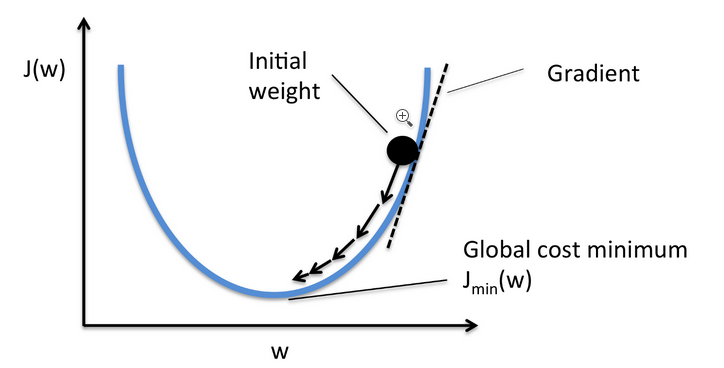
\includegraphics[scale=0.65]{img/gradient.png}
    \caption{How the backpropagation works}
    \label{img:gradient}
\end{figure}

So the idea is we needs to adjust each parameters in a model in order to minimize the loss. In order to automatize this process we need a technique that determines for each parameter if it needs to be raised or lowered. This technique is called \textbf{Back Propagation of the Gradient}. The idea is: the derivative of a function respect a variable tells us if moving forward or backward that variable the output of the function will raise or decrease.  The is exactly what we need. 

Let's define the \textbf{Gradient} as the vectors that contains the partial derivative of each parameters respect the loss function. If the partial derivative is positive so we know that, in order to lower the loss, we need to reduce the value of that parameter otherwise we need to raise the value of that parameter. Geometrically the gradient is the vector that points to the direction where function raise most. 
So the update step is doing by:
\begin{equation}
w_i^t = w_i^{t-1} + \alpha\bigtriangledown_{wi} 
\end{equation}
where $w_i^t$ is the weight $i$ at the time $t$, $\bigtriangledown_{wi} $ is the gradient of the function, in this case it represent the partial derivative of the loss function respect the parameter $wi$. The $\alpha$ represent how much the weight will be incresed or decreased. This value is called \textbf{Learning Rate}



So this is the overview on how weight are update but what is an Optimizer?
The optimizer is the selected technique to update weight, the Back propagation of the Gradient is a technique but also the basic technique, the others will extend this concept in order to make the process faster.

\subsection{}


\chapter{Markov Decision Processes}
Paper: A survey of Application of Markov decision processes
Paper: Markov decision Process: concepts and algorithms

\chapter{Generative Models}
In this chapter I'm gonna put all stuff about generative field. I'd lie to speak about GANs network and other advanced stuff but before I need to put together some backgrounds concepts like Boltzman machine Energy-based model and so on. 

\section{Energy based model}
%This is an extract of the presentation \textit{https://deepgenerativemodels.github.io/assets/slides/cs236\_lecture11.pdf}
Let's say that a probability function $p(x)$ needs to respects this rules:
\begin{itemize}
 \item $\forall x, p(x) >= 0$ 
 \item $\sum_x p(x) = 1$
 \end{itemize} 
 You can have a more deep definition in the probability chapter.
 In order to define this $p(x)$ function we need to guarantee the respect of those constrains. Let's imagine $p(x) = x^2$
 In this case the first rule is respected but not the second, so this function can be used. So, to use a positive function we need to normalize it. Let's define $p'(x)$ as the normalized version of $p(x)$ in order to respect both the rule:
 \begin{equation}
 p'(x) = \frac{p(x)}{\int p(x)dx}
 \end{equation}\label{normalizationfunctionforprobability}
 We have normalized $p(x)$ by the area above the the function.
 
 Now we can define  the probability function $p(x)$ the function:
 \begin{equation}
 p(x) = \frac{exp(f(x)}{\int exp(f(x))dx}
 \end{equation}
 We can define:
 \begin{equation}
 Z = \int exp(f(x))dx
 \end{equation}
 As you can see it was used $exp()$ function in order to guarantee the first rule. Furthermore this function allow to better capture variations, many distribution can be written in exponential form.
 
 In this system we can call $f(x)$ the \textbf{The energy function} and we see the method to turn it in to a probability function
 
\subsection{How it work?}
 The \textbf{Energy based model} has to associate to each configuration of the input variables a scalar that indicates how much energy has this configuration. A good configuration has low energy, so a low value while a bad one has a greater energy.
 
 For example let's say we have in imagine $M$ and a set of object $(s_0, s_1,.. s_5)$. The imagine contains one object from the set and we want create a model capable to identify it. Let's say that we want a model capable to give to the right $s_i$ lesser energy than the other.
 
  %https://rubikscode.net/2018/10/01/introduction-to-restricted-boltzmann-machines/
 \section{Boltzman Machine}
 \begin{figure}
  \centering
    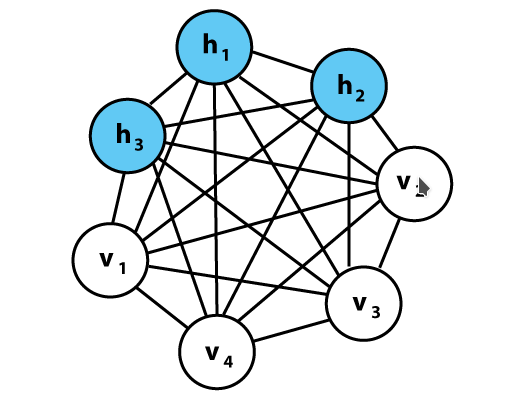
\includegraphics[scale=0.65]{img/boltzmanMachine.png}
    \caption{boltzman machine model}
    \label{img:bolzman_machine}
 \end{figure}
 Boltzman machine is a symmetrically  connected neurons model. Each of these neurons has a binary state so they can be on or off.
 A Boltzman machine is composed by nodes, called, neurons, connected to the others with a weighted connection. Nodes can be visible of hidden. This means the user will be able to set input in the visible neurons not in the hidden ones.
 
 Each neurons compute its state according to a probability function that means the probability of the neuron to change state:
 
 \begin{equation}
 prob(s_i = 1) = \frac{1}{1 + e^{-z_i}}
 \end{equation}
 
 As we can see this formula uses a parameter $z_i$ that is computed by summing all weighted states of input nodes plus a bias:
 
 \begin{equation}
 z_i = b_i + \sum_{j} s_j w_{ij}
 \end{equation}
 
 Now, once all nodes are update, we can compute the \textbf{Energy of the system} using a \textbf{Boltzman Distribution} that is a energy probability function for discrete value.
 
 Let's define $\vec{v}$ the vector containing all states and $\mathbb{U}$ all the possible state vectors. Now we can compute the probability of the system using:
 \begin{equation}
 P(\vec{v}) = \frac{exp(-E(\vec{v}))}{\sum_{\vec{u}\in\mathbb{U}} exp(-E(\vec{u}))}
 \end{equation}

$E()$ is the boltzman energy function:
\begin{equation}
E(\vec{v}) = - \sum_i s_i^v b_i - \sum_{i < j} s_i^v s_j^v w_{ij}
\end{equation}

The goal of this machine is to set weighs in order to minimize the energy of the system for the right configuration of states, and maximize it for the wrong configuration.
\textbf{Problems:} Nodes are all connected to each other and that makes the model learning really long. That why \textbf{Restricted Boltzman Machines (RBM)} came into the picture

\subsection{Restricted Boltzman Machine}
\begin{figure}
  \centering
    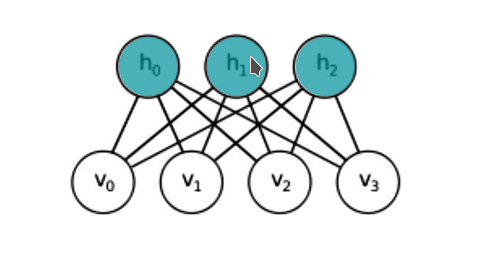
\includegraphics[scale=0.65]{img/RestrictedBoltzmanMachine.png}
    \caption{restricted boltzman machine model}
    \label{img:restricted_bolzman_machine}
 \end{figure}
 The main difference between Boltzman Machine and Restricted Boltzman Machine is that visible nodes are link just to hiddens one and viceversa. Less connections less learning time. The State vector $\vec{v'}$ is composed by the visible state vector $\vec{v}$ and the hidden vector $\vec{h}$. The energy is computed:
 \begin{equation}
 E(v,h) = - \sum_{i} a_iv_i - \sum_j b_j h_j - \sum v_i h_i w_ij
 \end{equation}
Where $a_i$ and $b_i$ are the bias. The probability of the system can be expressed as:
\begin{equation}
p(v,h) = \frac{exp(-E(v,h))}{\sum_{v,h} exp(-E(v,h))}
\end{equation}
Now it si possible to calculate the probability of a single hidden neuron to be activated:
\begin{equation}
p(h_j = 1 | v) = \frac{1}{1 + exp(-(b_j+W-jv_j))} = \sigma (a_i + \sum_j h_j w_ij)
\end{equation}

As we can see from the above equation it can be expressed as a logistic function

\chapter{EXTRA: Neural Symbolic Integration}
\section{Introduction to Neural Symbolic Integration}
Well, it is a real chaos out there but let's try to put things together. With \textbf{Neural Symbolic Integration} we mean the set of techniques used to combine Symbolic Approach with Neural network Approach. At the very beginning of the AI (1970 more or less) there were two different directions: \textbf{Symbolic AI} and \textbf{Connectionist AI} (or sub-symbolic). The former wants to explain the knowledge and the reasoning to get a task done by using Logic Rules as Prolog, or Descriptive Logic (Cond, Cond => State). The latter, on the other hand, wants to get best results with less effort. From this direction was born Machine Learning and in particular Deep Learning.

So, on one hand we have symbolic approaches that are clear, transparent but less precises, less powerful, less applicable in real context due to scalability, distribution and so on. Those approaches are based on Logic (Symbols, Relation between them, abstract connection) and the manipulation of them and this approach is considered \textit{Top-Down} knowledge is from abstract representation using Logic and not in raw data and experience.

 On the other hand we have connectionist approaches or sub-symbolic approaches that totally lacks of transparency but they can handle big data, they can scale and be distributed, they are power with good result. They also lack of a real reasoning. This approach use statistical function to extract information from raw data so it is called \textbf{Bottom-Up} because knowledge comes from raw data. They learn trough experience.

So the \textbf{Neural Symbolic Integration} is the research fields that studies technique to put them together and get the most from both. The field also called Neural Symbolic Computation is one of the many that exist but it is the most promising so we speak about it as the only one. This field obtained new interesting by the research community very recently so it lacks of common tasks, common formalism and also common objectives that can make possible clear comparison between solutions. There are a lot of different solutions in the wild very different and the only thing in common is they try to put some logic with neural network.

But in this heterogeneous mixing we can cluster solution in two groups:
\begin{itemize}
  \item  \textbf{Logic as Constrain} where logic is inserted directly into the neural model that to guide the training process, working as regularization factor. In this way a trained network has high-level knowledge inside.
  \item \textbf{Differentiable Programming} or \textbf{Logic as Task}. The idea is to create a mapping between logic and numerical domain in order to use Neural network on the second to solve problems in the first. Logic guides the construction of an Equivalent Neural Network. 
  \end{itemize}  


\subsection{Logic As Constrain}
%%todo
\subsection{Logic As Task}
%%todo


 
 \section{Neural Symbolic Cognitive Agent (NSCA) }
 from paper \textit{A Neural-Symbolic Cognitive Agent for Online Learning and Reasoning}.
 The first point is existing models are too simplified and require too time to be used in online learning and reasoning. Furthermore, some high-order concepts have temporal relation hard to represent by hand. They propose a new model capable to learn new hypotheses from observed data in complex environment. More precisely the model is able to:
 \begin{itemize}
  \item Perform learning of complex temporal relations from uncertain observations
   \item Reason probabilistically  about the knowledge learnd
   \item Represent the  agent's knowledge in a logic-based format for validation purposes.
  \end{itemize} 
  It takes advance of Statistical learning and Symbolic Representation
  
  
 \subsection{References}
 \textit{https://arxiv.org/pdf/1905.06088.pdf} - Neural-Symbolic Computing: An Effective Methodology for Principled Integration of Machine Learning and Reasoning


\chapter{Reinforcement Learning}
This chapter is my notes from a Udemy Course called \textbf{Deep Reinforcement Learning 2.0}. During the course I will see theory notions but implementations of some AI that keeps learn. I will face Q-Learning and other cool stuff.

The structure of the course will be:
\begin{itemize}
\item Extra theory
\item Foundamentals
\item Twin Delayed DDPG - Theory
\item Twin Delayed DDPG - Implementation
\end{itemize}

\section{Resources}
\url{https://arxiv.org/pdf/1802.09477.pdf}. It is the paper that we will discuss dring the course


\section{Extra theory: basic knowledge}

In this section we will see what is reinforcement learning, Bellman equation, Markov decision process, plans,  living penalty, q-learning, temporal difference.

\subsection{Reinforcement Learning}
 The main ingredients of a RL systems are:
 \begin{itemize}
 \item Agent: the AI that has to fulfill  a task by taking actions
 \item Environment: the place where Agent lives
 \item Action and rewards: mechanism that make Agent do thing and discriminate if it is right or not. Action are hard coupled with time.. a correct action in a wrong time leads a bad rewards.
 \end{itemize}
 
 Training AI is like training a dog, if it does right it get a reward otherwise nothing.
 
 \begin{figure}
    \centering
    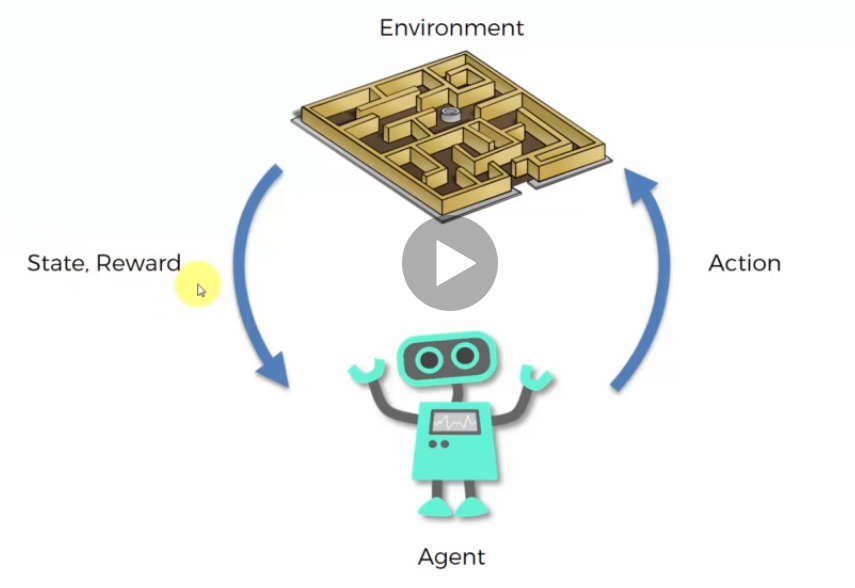
\includegraphics[scale=0.65]{img/reinforcementlearning01.png}
    \caption{Overview of Reinforcement Learning system}
    \label{img:RL-System}
\end{figure}

RL create RL agents that differs from Pre-Programmed Agents by the knowledge they have inside before start learning. The PPAgents have a series of rule that describe all actions they can do, in which case etc etc... while RL has to figure out those rule, his own behavior.

\subsection{BellMan Equation}

Notions:
\begin{itemize}
 \item $s$ the state of the agent
 \item $a$ action that agent can make
 \item $R$ reward agent gets for entering in a State
 \item $y$ Discount. 
 \end{itemize} 
 
  \begin{figure}
    \centering
    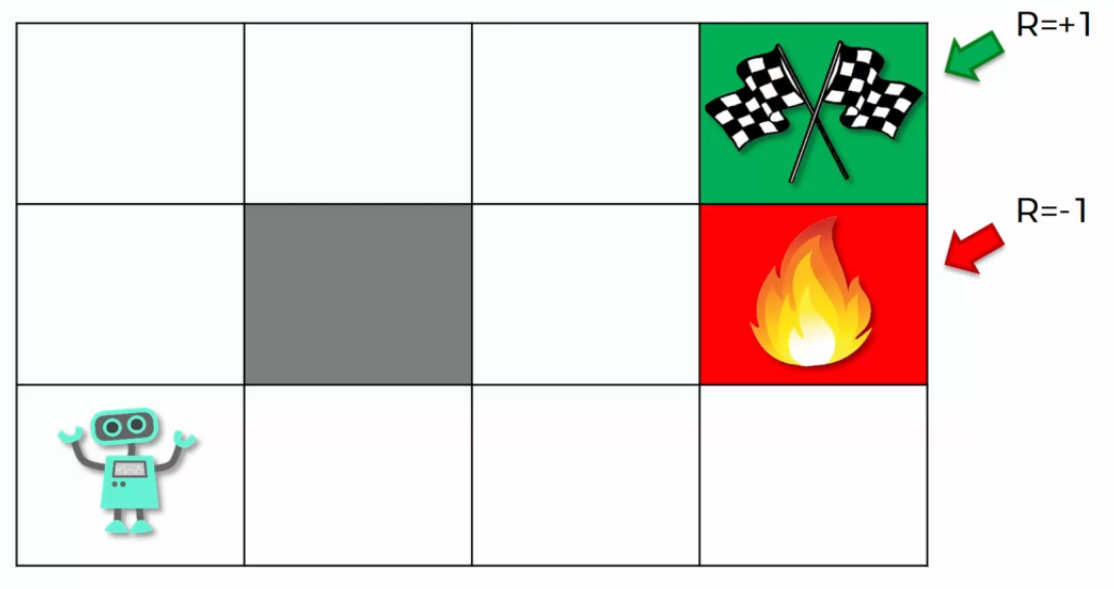
\includegraphics[scale=0.35]{img/rl-maze.png}
    \caption{RL - Maze task}
    \label{img:RL-Maze}
\end{figure}

 Before start let's define a task. We have an agent (the robot) in a maze composed by a grid with three different kinds of cells:
 \begin{itemize}
 \item Empy: the withe cell where agent is free to go
 \item Grey: the wall, agent cant cross this cell
 \item Red: The fire, agent can go there but it loses
 \item Green: the target, agent can go there and it wins
 \end{itemize}
 You can see this amazing maze in the picture \ref{img:RL-Maze}
 The agent can do 4 actions:
 \begin{itemize}
 \item Go Up
 \item Go Down
 \item Go Right
 \item Go Left
 \end{itemize}

\textbf{Basic Idea Of Bellman equation}. When agent goes to the green cell it gets a +1 rewards. It likes rewards, it is addicted, it cant live without so it think: "how i get the reward?" in order to be able to get it each time. So it learns that from the previous cell (3,3) it has to just move right (4,3) and he get the +1. Now each time it goes in (3,3) he knows how to get reward. He is happy but he could be more happy, more addicted. He start to think: "how i get here in the (3,3)" in order to be able to get this cell every time. So it learn for example that it can reach this cell from (3,2). Then it ask the same until it has learned a path from the start point to the green cell. Now it is really happy. 

\textbf{The bellman equation}. This is the bellman equation:
\begin{equation}
V(s) = max_a(R(s,a) + yV(s'))
\end{equation}
This equation gives a value $V$ to a State $s$ reached by the agent. The value is based on the best action it can take from that state. Let dig into it. We know agent in a state can take actions $a$, in our case it can chose between 4 actions each of them leads the action is a new state $s'$. Each action, took in a state has a reward for example if agent is in (3,3) and it goes right it get +1 as reward, if it is in (3,2) and it goes right it get -1 as reward because it ends in the fire. So each action, according to the current state, leads to different rewards $R(a,s)$. In the bellman equation we select the action that give the maximum value. So we cycle on all possible action computing the reward $R(s,a)$ and we select the action that brings agent to the greatest reward. We also consider the value of the reached state. Take an action brings agent from $s$ to $s'$ so the value of $s'$ must be taken in account $yV(s')$. So for each action we compute the reward $R(s,a)$ plus the value of the reached state $yV(s')$ and we select the action that gives the agent the greatest value because we want agent be optimal, so we can consider just best solutions.

\textbf{Let's do some example}
Let's compute the $V(s)$ of the (3,3) using a $y = 0.9$.
$V((3,3)) = R((3,3), goRight) + yV((3,4))$. We already know the best action because it is the only action that leads agent to the target (3,4). So considering this action we compute the value.

$V((3,3)) = 1 + y0$ V(3,4) is zero cause it is the target cell and we don't need it to have a value
So $V((3,3)) = 1$

We can repeat this for the V(2,3), we know the best action is go right so $V(2,3) = 0 + 0.9 * 1 = 0.9$. We can repeat the it for each cell.

\begin{figure}
    \centering
    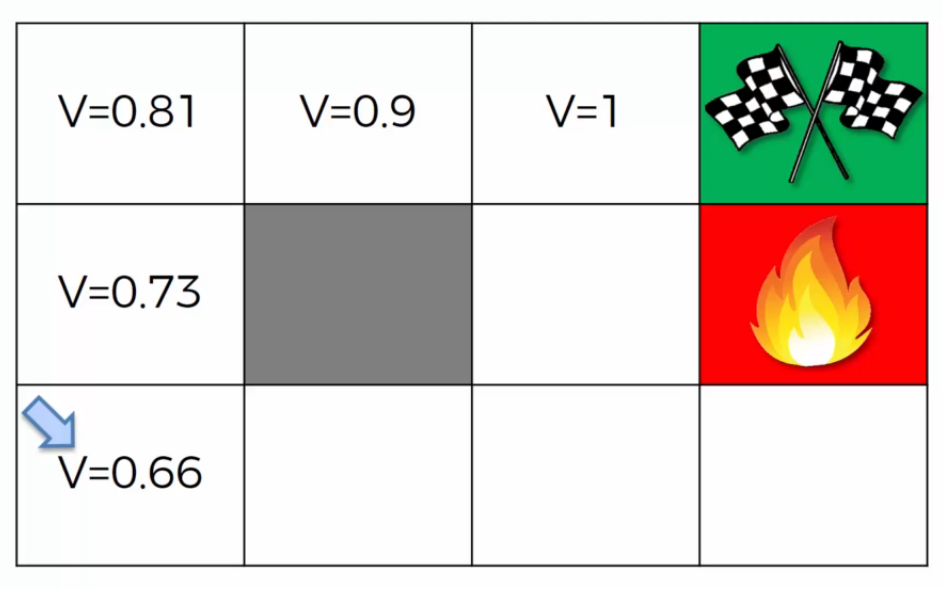
\includegraphics[scale=0.35]{img/rl-maze-be.png}
    \caption{RL - Maze task with values from bellman equation}
    \label{img:RL-Maze}
\end{figure}

It easy to see that value decreases according to the distance to the target cell (4,3).

\subsection{Stochastic variable... OMG}
Untill now we speak about the maze a a very kind one. U want to go up, then u go up with 100\% possibility. But this is not how real life, out there, works. Let's add some randomness, let's create a stochastic maze where the action is a stochastic process. For example in cell (2,3) ground is broken so if u want to go up you have: 
\begin{itemize}
\item 80\% of probability to go up
\item 10\% of fall down
\item 10\% of fall in the cell with the hell's fire and die.
\end{itemize}

This is a \textbf{Markov Process} because the state $s'$ is expressed just according to the current state and not the previous decision of the agent. (Check the chapter about Markov Process).

That is how real work works. Our robot, that is addicted wish to get to the cell (3,3) because it perfectly know how to reach is drug from there. So from (3,2) decide to go up but it risk to fail and worsening his position. So the value of this cell must decrease.

Let's define the new Bellman Equation considering the Markov Decision Process:
\begin{equation}
V(s) = max_a(R(s,a) + y \sum_{n} P(s,a,s'_n)V(s'_n))
\end{equation}
Let's explain that, now agent can end in different states $s'_1 s'_2 ... s'_n$ and it can end there with a certain probability. Let's define P() as a function that gives to us this probability:
$P(s,a,s'_n)$ gives to us the probability from $s$ to reach $s'_n$ by action $a$. For each possible state $s'_n$ we need to compute this probability and multiply it with the value of that state and sum all values obtained.

Let's do an example. Let's compute the value of (3,2) considering the hard ground.
$V((3,2)) = 0 + 0.9 * ((0.8 * 1) + (0.1 * 0.73) + (0.1 * -1)) = 0.6957$

\begin{figure}
    \centering
    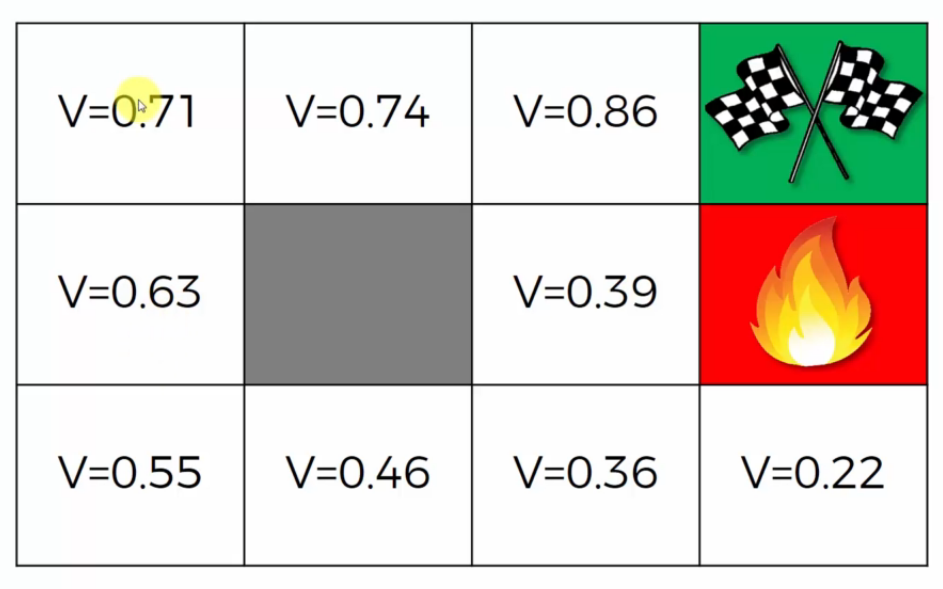
\includegraphics[scale=0.35]{img/rl-maze-stoch.png}
    \caption{RL - Maze task with all values changed because in each cell there is a probability to fall in two wrong cells}
    \label{img:RL-Maze-stoch}
\end{figure}

From pics \ref{img:RL-Maze-stoch} it's possbile to see the new cell values considering the probability to end in the wrong cells (80\%, 10\%, 10\%). That is why the agent in the cell (3,2) wont try to go up because he know that he have 10\% of probability to end in the fire an die. But it is more convenient for him to try to go in the wall an stay in the cell (3,2) but have a 20\% of probability to fall in a better cell without risk to end in the fire. It's possible to see it in the picture \ref{img:RL-Maze-plan}.

\begin{figure}
    \centering
    \includegraphics[scale=0.35]{img/rl-maze-plan.png}
    \caption{RL - Maze task with all values changed because in each cell there is a probability to fall in two wrong cells. We can see the actions that agent will try to take in each cell}
    \label{img:RL-Maze-plan}
\end{figure}

\subsection{Rewarding}

In our maze, by now, agent get two rewards the +1 if it arrives in the (4,3) cell (the green) or -1 if it ends in the fire. But what takes the agent away from waste time? Maybe it wants to walk a bit before get the reward? But we want agent be more addicted possible, we want it suffering the pain of hell if it doesn't get fast his drug!! Let's introduce \textbf{The Living Penalty}, a negative reward that it gets each time it take and actions. More action it takes more penalty if collects. Using this it select different action, for example it stops to try to go in the wall, has it does without penalty. You can see this differences in the picture \ref{img:RL-Maze-LP} 

\begin{figure}
    \centering
    \includegraphics[scale=0.35]{img/rl-maze-LP.png}
    \caption{RL - Actions for the maze with different Living Penalty}
    \label{img:RL-Maze-LP}
\end{figure}

\subsection{Q-Learning}
By now, using bellman equation, the best action is chosen by knowing the value of a state and selecting the action that brings agent it that state. In Q-Learning approach the idea is to evaluate directly the action using a \textit{Quality function} to measure the quality of an action $Q(s, a)$ where $s$ is the state of the agent  and $a$ is the action.
The $Q(s,a)$ equation come from this equation:
\begin{equation}
Q(s,a) = R(s,a) + y \sum_{n} P(s,a,s'_n)V(s'_n)
\end{equation}

As we can see it is identical to the final piece of bellman equation. But we still have $V(s)$ in our equation and we don't want it because it focuses on value of state and we want focus on value of possible action:

\begin{equation}
Q(s,a) = R(s,a) + y \sum_{n} P(s,a,s'_n) max_{a'}Q(s'_n, a')
\end{equation}

\subsection{Temporal Difference}

Now it obvious ask ourselves  if the same action at different time can have different value or precisely different q-function results. Let's introduce the temporal difference concept.

\textbf{Intuition}. Let's say our agent is for the first time in the maze. Let's place him in (1,1) at the very start. Now he can go in both direction (2,1) o (1,2). By now he has no idea of the path for the reward so he evaluates them equally: $Q(a_0, s) = Q(a_1,s)$. After some exploration he is back in the first cell (1,1). The cell is the same as before, the possible actions are the same as before but now he knows the best path so $Q(a_0, s) > Q(a_1,s)$. That means that $Q_{t_0}(a_0, s) < Q_{t_n}(a_0,s)$ because agent learned the best path. The same action from the same cell can have different importance according to the time it is performed because agent learn at each time.

Let's define this concept introducing $t$ the time:
\begin{equation}
Q_{t_1}(s,a) = Q_{t_0}(s,a) + { Q_{t_1}(s,a) - Q_{t_0}(s,a) }
\end{equation} 
From the above equation we can see that the $Q$ at time $t$ is the $Q$ at time $t-1$ plus the difference between them. Very easy .. doesn't it?. This difference is what agent has learned.
Let's call $Q_{t_1}(s,a) - Q_{t_0}(s,a) = TD(s,a)$ the temporal difference between the same action $a$ in the same state $s$ but in different times. We can now rewrite the equation as:
\begin{equation}
Q_{t_1}(s,a) = Q_{t_0}(s,a) +\alpha TD(s,a)
\end{equation}
$\alpha$ is a parameter that tell to the agent how much care to the past $Q_{t_0}$ or to the knowledge learned $TD$
In order to better understand let's expand the equation:
\begin{equation}
Q_{t_1}(s,a) = Q_{t_0}(s,a) + \alpha(R(s,a) + max_a Q(s',a') - Q_{t_0}(s,a))
\end{equation}
From this equation we can see that if $\alpha$ is set to 1 we have this:
\begin{equation}
Q_{t_1}(s,a) = R(s,a) + max_a Q(s',a')
\end{equation}
So the entire old value of $Q_{t_0}$ is replaced be the new value that comes from what agent has learned ( that is inside: $max_a Q(s',a')$). Otherwise, if we put $\alpha$ to 0 we 
 have:
 \begin{equation}
Q_{t_1}(s,a) = Q_{t_0}(s,a)
\end{equation}
From this equation we can see that nothing has changed so agent has learned nothing. This means that $\alpha$ is a coefficient that weight how much agent has to update its knowledge according to his new discoveries. Let's call $\alpha$ \textbf{learning rate} and this process \textbf{Q-Learning Process}. At the beginning of this process $Q(s,a)$ will be very low (or wrong) and the $TD$ very high. After some passages, when agent has learned the optimal path so the optimal action $Q(s,a)$ will be high (or optimal) and $TD$ will be low because agent can't learn something new.

\section{Deep Q-Learning}
\begin{figure}
    \centering
    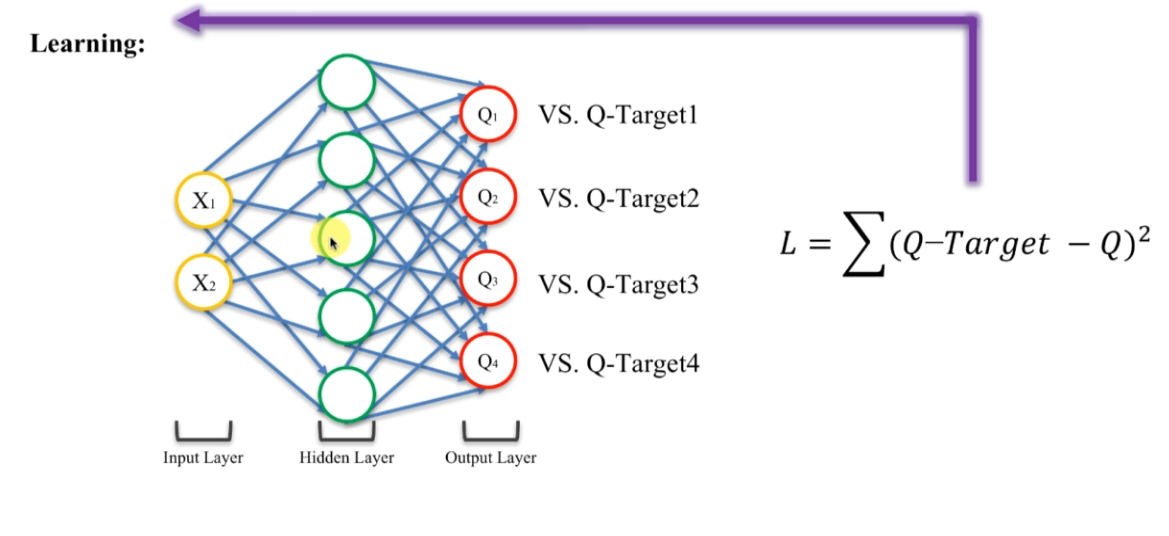
\includegraphics[scale=0.45]{img/rl-deepql1.png}
    \caption{RL - Deep Neural Network overview for deep q-learning}
    \label{img:RL-deep-ql}
\end{figure}

The idea of \textbf{Deep Q-Learning} is to use a neural network to learn the best action to do in a given place. So the model should take in input $s$ expressed as a pair $<x_0, x_1>$ and it tries to predict the right action. So it gives in output a vector $<q_0, q_1, q_2, q_3>$ that represent the q-learning value associated to each action. \textit{This algorithm (deep q-learning) can be applied just when you have discrete actions like in this case.}

\subsection{Experience Replay}

The agent performs some actions and save them in a memory as experience. Then it select some of the past action, using a uniform distribution, and evaluate them. 

\texttt{To read: Prioritized Experience Replay - google deepmind 2016}

Experience Replay has different implementation so we have to define some policies like: max number of experience to save, how to discharge past experience for new ones, how to select them etc etc. 

\subsection{Action Selection Policy}
%% to do

\subsection{Deep Q-Learning: The algorithm}

First of all we need to put agent in a context. Then we need to define \textbf{Experience Replay Policy} and we are ready to start. So our agent will be in a state $s$ and he can do the same 4 actions: up, down, right, left. So he will try to do the best action predicting the Q-Value for each possible action. Let's say he predicts $[Q^p(s,up), Q^p(s,down), Q^p(s,right),Q^p(s,left)]$. The first time he will predict random value for instance: $[0.1, 0.1, 0.4, 0.05]$. According to our action selection policy he will select one action to do, let's say it select the one with the best score so: right. Now agent moves right and enters in a new state $s'$. Let's say he also get a reward $r = 1$ so now he can compute a better q-value for the action $right$ from state $s$: $Q^t(s,right) = R(s, right) + ymax_aQ(s', a) = r + 0 = 1$. Now agent can save in memory the experience using the tuple $(state = s, action = right, reward = r, end_state = s')$, for clarity let's express this tuple using time because agent can experience the same situation more times so  $(state_t = s, action_t = right, reward_t = r, end_state_t = s')$. He also save for that experience the predicted q-values.


It's time for the agent to learn. He predicted for this action the q-value $Q^p_{right} = 0.4$ then he performed the action and he discovered that a more precise q-value was $Q^t(s,right) = 1$ so he can use the loss function $Loss(Q^p, Q^t) = (Q^t - Q^p)^2$ and than he can back-propagate the gradient of the function to update weights as in a normal Neural Network.

 Let's add a new complexity, the memory. When agent has to learn he doesn't use just that experience but he select from his memory also N - 1 past experiences $e_0, e_1,..., e_{n - 1}$. He adds the new experience he has just performed and he get a pool of N experiences. Now it try to learn also form those experiences using the loss function:
 \begin{equation}
 Loss = \frac{1}{2} \sum_e ((Q^t(s,a) - Q^p_e(s,a))^2
 \end{equation}
 \newpage
 \section{Formula Summary}
 Bellman Equation:
 \begin{equation}
 V(s) = max_a(R(s,a) + yV(s'))
 \end{equation}
 Bellman Equation in a Markov Decision Process:
 \begin{equation}
 V(s) = max_a(R(s,a) + y \sum_n P(s,a,s'_n)V(s'_n))
 \end{equation}
 Q-Learning Equation:
 \begin{equation}
 Q(s,a) = R(s,a) + y \sum_n P(s,a,s'_n)V(s'_n) = R(s,a) + y \sum_n P(s,a,s'_n)max_{a'}Q(s'_n, a')
 \end{equation}
 Q-Learning Equation simplified (\textit{This equation substitutes the previous just because it is shorter, for simplicity}):
  \begin{equation}
 Q(s,a) = R(s,a) + ymax_{a'}Q(s'_n, a')
 \end{equation}
 
 
 
 Temporal Difference:
 \begin{equation}
 TD(s,a) = Q_{t1}(s,a) - Q_{t0}(s,a)
 \end{equation}
 \begin{equation}
 Q_{t1}(s,a) = Q_{t0}(s,a) +\alpha(Q_{t1}(s,a) - Q_{t0}(s,a)) =  Q_{t0}(s,a) +\alpha TD(s,a)
 \end{equation}
 \begin{equation}
 Q_{t_1}(s,a) = Q_{t_0}(s,a) + \alpha(R(s,a) + max_a Q(s',a') - Q_{t_0}(s,a))
 \end{equation}
 

 
\end{document}


